\section{Estado del Arte}

Desde el año 2002, proyectos de VO's comenzaron a integrar
la Alianza Internacional Observatorio Virtual bajo el \textbf{Guidelines
for Participation\footnote{La documentación se puede
encontrar en \url{http://www.ivoa.net/documents/latest/IVOAParticipation.html}}}.

Estos fueron fundados bajo programas privados y gubernamentales nacionales e
internacionales en colaboración con centro de estudios científicos,
universidades y otros. Quienes integran este proyecto, el Observatorio Virtual, 
comparten conocimientos entre ellos y la comunidad de modo estandarizado. Son 
ellos mismos quienes desarrollan estos estándares para el intercambio de 
información e interoperabilidad.

El cuadro \ref{table:integrantes} muestra los miembros de IVOA hasta mayo de
2013

\begin{table}[h!t]
	\centering
	\begin{tabular}{l} \hline
		%\hline
		\textbf{Proyecto} \\\hline
			Argentina Virtual Observatory\cite{arg} \\
			Armenian Virtual Observatory\cite{arm}\\
			AstroGrid\cite{astrogrid}\\
			Australian Virtual Observatory\cite{aus}\\
			Brazilian Virtual Observatory\cite{bra}\\
			Canadian Virtual Observatory\cite{can}\\
			Chinese Virtual Observatory\cite{china}\\
			European Space Agency\cite{esa}\\
			European Virtual Observatory\cite{euro}\\
			German Astrophysical Virtual Observatory\cite{ger}\\
			Hungarian Virtual Observatory\cite{hun}\\
			Italian Virtual Observatory\cite{ita}\\
			Japanese Virtual Observatory\cite{jap}\\
			Observatorie Virtual France\cite{fra}\\
			Russian Virtual Observatory\cite{rus}\\
			Spanish Virtual Observatory\cite{spa}\\
			Ukranian Virtual Observatory\cite{ukr}\\
			Virtual Astronomical Observatory\cite{usa}\\
			Virtual Observatory India\cite{ind}\\
            \hline
	\end{tabular}
	\caption{Integrantes de IVOA}
	\label{table:integrantes}
\end{table}

Casi la mitad de los observatorios virtuales de IVOA están en Europa: 9 del
total; 1 pertenece a Oceanía, 4 a América y 5 de ellos a Asia \footnote{Como la
mayor parte de Rusia está en territorio Asiático, es considerado como uno de
los VO's de ese continente.} La figura 1 muestra la distribución de los
miembros de IVOA por continente.
	\begin{figure}[h!t]
		\begin{center}
			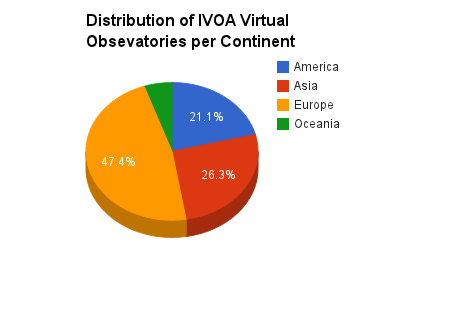
\includegraphics[width=0.5\textwidth]{img/ivoa_vos_distribution.png}
			\caption{Distribución por continente de IVOA.}
		\end{center}
	\end{figure}

Si Chile se convirtiera en miembro de IVOA, la distribución de los miembros
por continentes sería la que se muestra en la figura 2.
	\begin{figure}[h!t]
		\begin{center}
			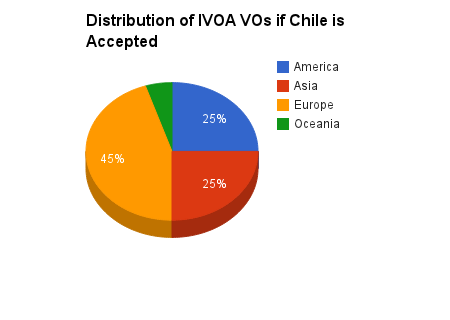
\includegraphics[width=0.5\textwidth]{img/if_chile_is_accepted.png}
			\caption{International Virtual Observatory Alliance Distribución por continente incluyendo a Chile.}
		\end{center}
	\end{figure}

Sin considerar el estado de los proyectos internos de los VO's, 
la membresía de Chile contribuiría a que América, llegue a la misma
cantidad en número de VO's que Asia. Por otra parte, este
hecho sería muy significativo, ya que un gran número de centros astronómicos
como los observatorios se instalan en este país. Por ahora, se pretende
trabajar con datos del proyecto ALMA. Actualmente se está realizando
un estudio de proyectos individuales que está ejecutando cada VO, sus resultados actuales
y los esperados.
